
Struktur kelas pada aplikasi \textit{Broken Link Checker} dibagi ke dalam tiga \textit{package} utama, yaitu \texttt{Web Crawling}, \texttt{URL Fetcher}, dan \texttt{GUI Manager}. \textit{Package} \texttt{Web Crawling} berisi kelas-kelas inti yang mengatur proses \textit{crawling}, pengelolaan \textit{frontier}, serta representasi tautan. \textit{Package} \texttt{URL Fetcher} menyediakan mekanisme untuk mengambil konten dari situs web menggunakan pustaka eksternal seperti Jsoup dan \texttt{HttpClient}. Sementara itu, \textit{package} \texttt{GUI Manager} menangani pengelolaan antarmuka pengguna dengan JavaFX, termasuk kontrol proses pemeriksaan dan penyajian hasil. Diagram kelas untuk aplikasi ini dapat dilihat pada Gambar~\ref{fig:class-diagram}.

Penjelasan setiap kelas pada diagram adalah sebagai berikut:

\begin{enumerate}
    \item \textbf{Kelas Link}\\  
    Kelas \texttt{Link} merupakan kelas dasar yang merepresentasikan sebuah tautan dalam sistem. Kelas ini menjadi induk bagi \texttt{WebpageLink} dan \texttt{BrokenLink}, sehingga relasinya berupa pewarisan.
    \begin{itemize}
        \item \texttt{url} : Atribut ini bertipe data \textit{String} dan digunakan untuk menyimpan alamat dari tautan yang diperiksa.
        \item \texttt{statusCode} : Atribut ini bertipe data \textit{int} dan berfungsi untuk menyimpan kode status HTTP hasil pemeriksaan tautan.
        \item \texttt{accessTime} : Atribut ini bertipe data \textit{Instant} dan merekam waktu terakhir kali tautan tersebut diakses.
    \end{itemize}

    \item \textbf{Kelas WebpageLink}\\
    Kelas \texttt{WebpageLink} merepresentasikan tautan yang termasuk dalam kategori halaman web dengan \textit{host} yang sama seperti URL awal. Kelas ini mewarisi \texttt{Link} dan memiliki relasi \textit{many-to-many} dengan \texttt{BrokenLink}.
    \begin{itemize}
        \item \texttt{brokenLinks} : Atribut ini bertipe data \textit{Map<BrokenLink, String>} dan digunakan untuk menyimpan daftar tautan rusak yang ditemukan di halaman beserta informasi anchor text-nya.
    \end{itemize}

    \item \textbf{Kelas BrokenLink}\\
    Kelas \texttt{BrokenLink} digunakan untuk menyimpan data tautan yang gagal diakses atau menghasilkan status \textit{error}. Kelas ini mewarisi \texttt{Link} dan memiliki relasi \textit{many-to-many} dengan \texttt{WebpageLink}.
    \begin{itemize}
        \item \texttt{webpageLinks} : Atribut ini bertipe data \textit{Map<WebpageLink, String>} dan digunakan untuk mencatat daftar halaman tempat tautan rusak tersebut ditemukan beserta lokasi anchor text-nya.
    \end{itemize}

    \item \textbf{Kelas Crawler}\\
    Kelas \texttt{Crawler} merupakan inti dari proses \textit{web crawling} dan bertanggung jawab mengelola antrean URL, melakukan pengambilan halaman, serta memeriksa status tautan. Kelas ini berhubungan langsung dengan \texttt{Frontier}, \texttt{WebpageLink}, dan \texttt{BrokenLink}, serta memiliki dependensi terhadap \texttt{Jsoup} dan \texttt{HttpClient}.
    \begin{itemize}

        \item \texttt{rootHost} : Atribut ini bertipe data \textit{String} dan digunakan untuk menyimpan host dari URL awal (seed URL).
        
        \item \texttt{frontier} : Atribut ini bertipe data \textit{Frontier} dan berfungsi sebagai antrean URL yang akan diproses.
        
        \item \texttt{repository} : Atribut ini bertipe data \textit{Set<String>} dan digunakan untuk menyimpan daftar URL yang sudah pernah dikunjungi agar tidak diperiksa dua kali.
        
        \item \texttt{USER\_AGENT} : Atribut statis ini bertipe data \textit{String} dan digunakan untuk mendefinisikan identitas permintaan HTTP yang dikirim oleh aplikasi.
        
        \item \texttt{TIMEOUT} : Atribut statis ini bertipe data \textit{int} dan menentukan batas waktu maksimum koneksi HTTP.
        
        \item \texttt{HTTP\_CLIENT} : Atribut statis ini bertipe data \textit{HttpClient} dan digunakan sebagai klien bawaan Java untuk mengirim permintaan HTTP.

        \item \texttt{Crawler} : Metode ini merupakan konstruktor yang menerima parameter \texttt{seedUrl} bertipe data \textit{String} dan digunakan untuk menginisialisasi proses \textit{crawling}.
        
        \item \texttt{startCrawling} : Metode ini menerima parameter \texttt{streamBrokenLink} bertipe \textit{Consumer<BrokenLink>} dan tidak mengembalikan nilai. Metode ini berfungsi untuk memulai proses \textit{crawling} dan mengirim hasilnya secara \textit{streaming}.
        
        \item \texttt{extractLinks} : Metode ini menerima parameter \texttt{doc} bertipe \textit{Document} dan mengembalikan daftar objek \texttt{BrokenLink}. Metode ini digunakan untuk mengekstrak seluruh tautan dari halaman HTML yang diambil.
        
        \item \texttt{normalizeUrl} : Metode ini menerima parameter \texttt{url} bertipe \textit{String} dan mengembalikan hasil normalisasi dalam bentuk \textit{String}. Metode ini digunakan untuk memastikan URL dalam format yang konsisten.
        
        \item \texttt{fetchUrl} : Metode ini menerima parameter \texttt{url} bertipe \textit{String} dan mengembalikan nilai \textit{int} yang merupakan kode status HTTP hasil pemeriksaan. Metode ini berfungsi untuk melakukan pemeriksaan tautan eksternal atau tautan umum menggunakan Java \texttt{HttpClient}.
        
        \item \texttt{isPotentialWebpage} : Metode ini menerima parameter \texttt{url} bertipe \textit{String} dan mengembalikan nilai \textit{boolean}. Metode ini digunakan untuk menentukan apakah suatu URL berpotensi merupakan halaman web.
    
    \end{itemize}

    \item \textbf{Kelas Frontier}\\
    Kelas \texttt{Frontier} berfungsi sebagai struktur data antrean (\textit{queue}) yang menyimpan URL yang akan diproses berikutnya. Kelas ini berelasi erat dengan \texttt{Crawler} yang mengelola antrean selama proses \textit{crawling} berlangsung.
    \begin{itemize}
        \item \texttt{urls} : Atribut ini bertipe data \textit{Queue<String>} dan digunakan untuk menampung daftar URL yang menunggu diproses.
        \item \texttt{enqueue} : Metode ini menerima parameter \texttt{url} bertipe \textit{String} dan berfungsi untuk menambahkan URL baru ke dalam antrean.
        \item \texttt{dequeue} : Metode ini tidak menerima parameter dan mengembalikan nilai \textit{String} berupa URL paling depan dari antrean.
        \item \texttt{isEmpty} : Metode ini tidak menerima parameter dan mengembalikan nilai \textit{boolean} untuk menunjukkan apakah antrean kosong atau tidak.
    \end{itemize}

    \item \textbf{Kelas Jsoup dan HttpClient}\\
    Kedua kelas ini merupakan representasi dari pustaka eksternal yang digunakan untuk melakukan pengambilan data web dan digunakan sebagai dependensi oleh kelas \texttt{Crawler}.
    \begin{itemize}
        \item \texttt{Jsoup} : Kelas ini digunakan untuk mengakses dan mengurai dokumen HTML dari halaman same-host dengan memanfaatkan parser HTML toleran kesalahan.
        \item \texttt{HttpClient} : Kelas ini digunakan untuk melakukan permintaan \texttt{HEAD} atau \texttt{GET} terhadap tautan umum atau eksternal untuk memeriksa status HTTP-nya.
    \end{itemize}

    \item \textbf{Kelas Controller}  
    Kelas \texttt{Controller} berfungsi sebagai penghubung antara logika aplikasi dengan antarmuka pengguna yang dibangun menggunakan JavaFX. Kelas ini berinteraksi dengan \texttt{Crawler} untuk menginisiasi dan menerima hasil proses pemeriksaan tautan.
    \begin{itemize}
        
        \item \texttt{seedUrlField} : Atribut ini bertipe \textit{TextField} dan digunakan untuk menampung input URL dari pengguna.
            
        \item \texttt{progressLabel} : Atribut ini bertipe \textit{Label} dan menampilkan status kemajuan proses pemeriksaan.
            
        \item \texttt{totalLinksLabel} : Atribut ini bertipe \textit{Label} dan menampilkan jumlah total tautan yang diperiksa.
        
        \item \texttt{webpagesLabel} : Atribut ini bertipe \textit{Label} dan menampilkan jumlah halaman yang berhasil di-crawl.
        
        \item \texttt{brokenLinksLabel} : Atribut ini bertipe \textit{Label} dan menampilkan jumlah tautan rusak yang ditemukan.
        
        \item \texttt{resultsTable} : Atribut ini bertipe \textit{TableView<BrokenLink>} dan menampilkan hasil daftar tautan rusak.
        
        \item \texttt{statusColumn} : Atribut ini bertipe \textit{TableColumn<BrokenLink, String>} dan digunakan untuk menampilkan kolom status pada tabel hasil.
        
        \item \texttt{urlColumn} : Atribut ini bertipe \textit{TableColumn<BrokenLink, String>} dan digunakan untuk menampilkan kolom URL tautan pada tabel hasil.
        
        \item \texttt{initialize} : Metode ini tidak menerima parameter dan berfungsi untuk melakukan inisialisasi awal saat antarmuka dimuat.
        
        \item \texttt{onStartClick} : Metode ini tidak menerima parameter dan digunakan untuk menangani event ketika pengguna menekan tombol \textit{Start}, kemudian memulai proses pemeriksaan tautan.
        
        \item \texttt{onStopClick} : Metode ini tidak menerima parameter dan digunakan untuk menghentikan proses pemeriksaan yang sedang berlangsung.
        
        \item \texttt{onExportClick} : Metode ini tidak menerima parameter dan digunakan untuk mengekspor hasil pemeriksaan ke dalam berkas Excel.
    \end{itemize}

    \item \textbf{Kelas Application}\\
    Kelas \texttt{Application} merupakan titik masuk (\textit{entry point}) dari aplikasi JavaFX. Kelas ini berhubungan dengan \texttt{Controller} untuk memuat dan menginisialisasi GUI.
    \begin{itemize}
        \item \texttt{main} : Metode ini tidak menerima parameter dan digunakan untuk menjalankan aplikasi.
        \item \texttt{start} : Metode ini menerima parameter \texttt{stage} bertipe \textit{Stage} dan berfungsi untuk memuat serta menampilkan antarmuka pengguna utama.
    \end{itemize}

    \item \textbf{Kelas HttpStatus}\\
    Kelas \texttt{HttpStatus} berfungsi sebagai kelas utilitas yang memetakan kode status HTTP ke \textit{reason phrase}. Kelas ini digunakan oleh \texttt{Controller} untuk menampilkan hasil status HTTP pada GUI.
    \begin{itemize}
        \item \texttt{STATUS\_MAP} : Atribut ini bertipe \textit{Map<Integer, String>} dan digunakan untuk menyimpan pasangan antara kode status HTTP dengan keterangan resminya.
        \item \texttt{getStatus} : Metode ini menerima parameter \texttt{statusCode} bertipe \textit{int} dan mengembalikan nilai \textit{String} berupa keterangan lengkap dari kode status tersebut.
    \end{itemize}
\end{enumerate}

\begin{figure}[H]
    \centering
    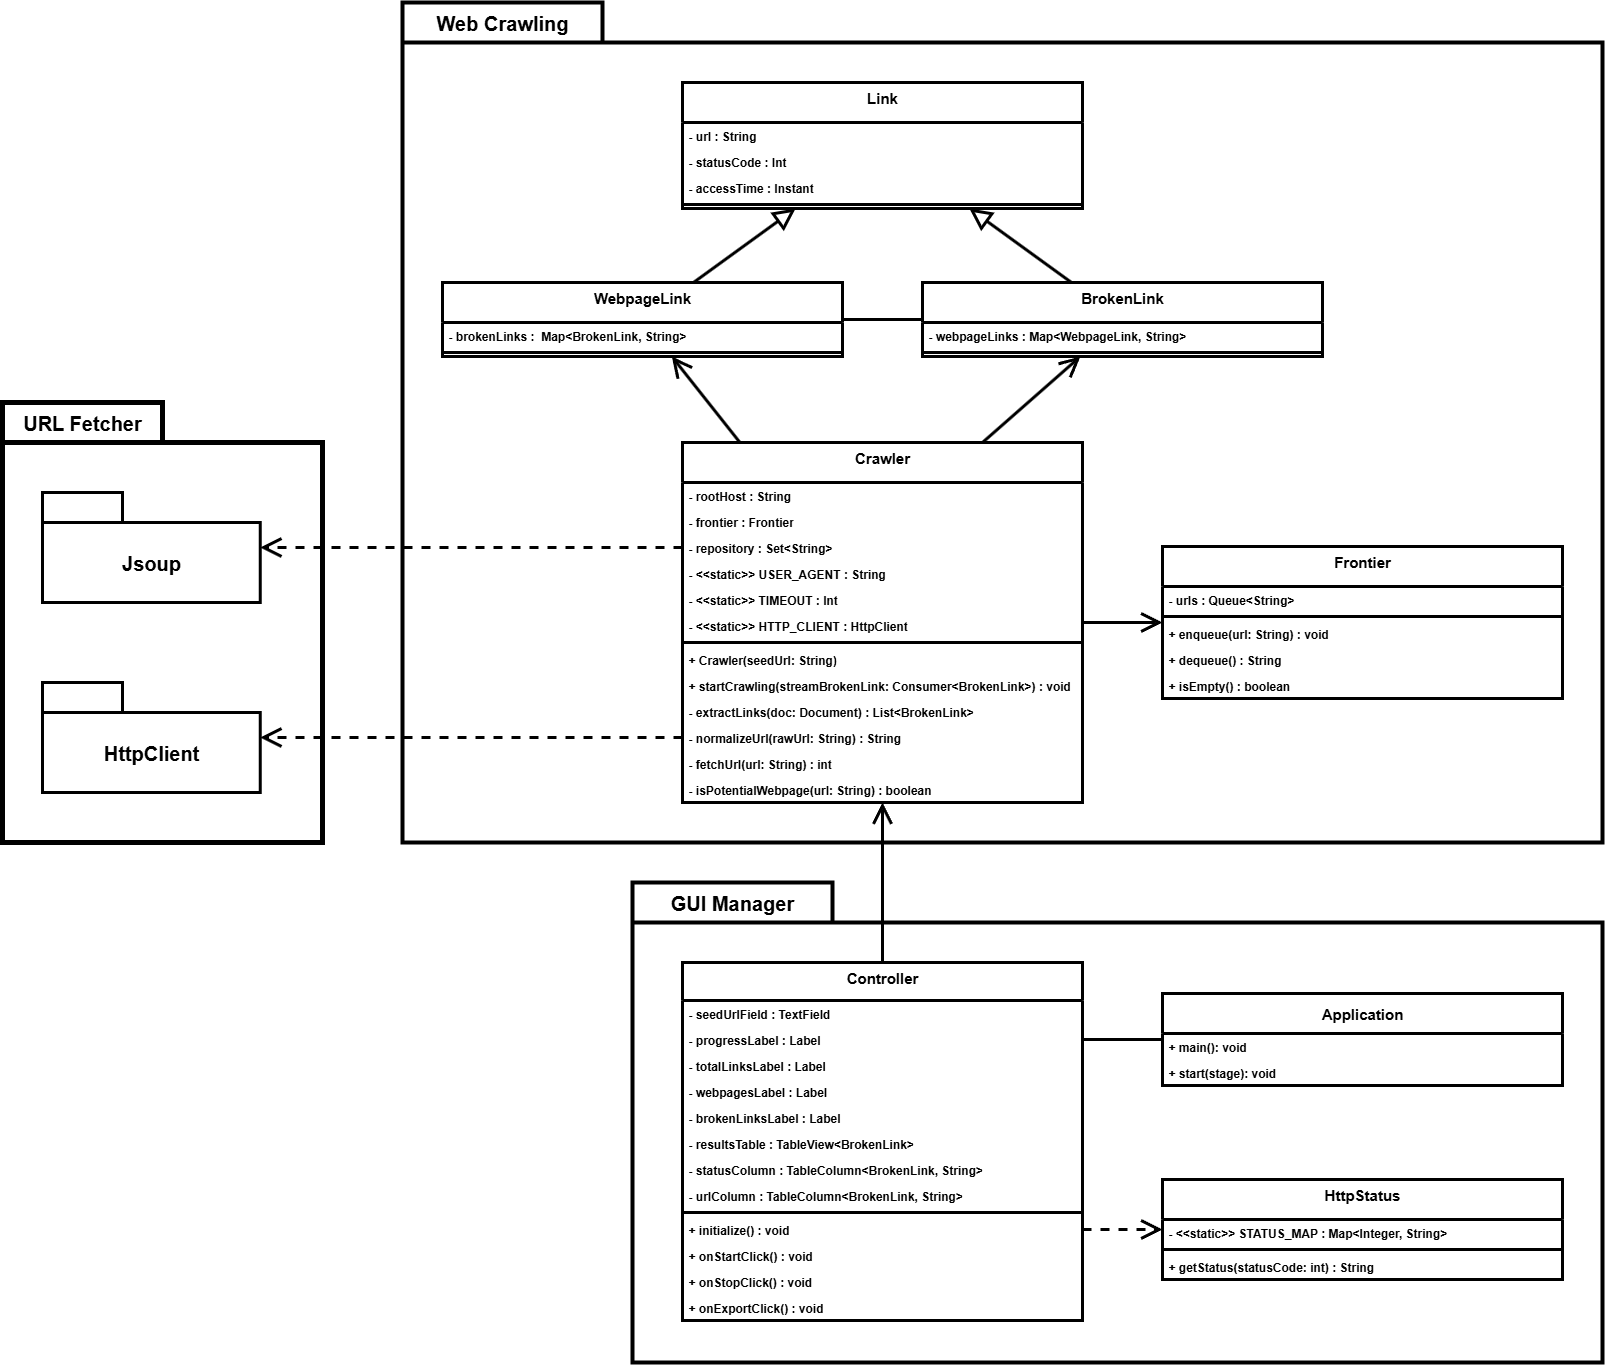
\includegraphics[width=0.95\textwidth]{Gambar/040100-class-diagram.png}
    \caption{Diagram kelas aplikasi}
    \label{fig:class-diagram}
\end{figure}